%% CAPITULO 1
\hypertarget{estilo:capitulo}{}
\chapter{INTRODUÇÃO} 

\section{Motivação}
\label{ss:motivacao}

A precipitação é um dos principais fenômenos da natureza que exercem grande influência na vida do homem e dos animais. Entende-se por precipitação toda a forma de água proveniente do vapor d'água da atmosfera e depositada sobre a superfície terrestre, como chuva, granizo, orvalho, neblina, neve ou geada (PINTO et al., 1976). A atmosfera atua como um grande reservatório de vapor d'água, o qual transporta e distribui a precipitação no planeta. Pode-se dizer que toda água que está sobre a superfície terrestre é resíduo das precipitações. A precipitação sob a forma de chuva além de ser mais facilmente medida, é a forma mais comum de precipitação e é a que mais contribui para a vazão dos rios na América do Sul (AS). 

A precipitação exerce grande impacto em diversos setores da atividade humana, como o planejamento agrícola, energético e hídrico, além de ser um fator determinante do clima e do tipo de vegetação característicos de diversas regiões. Além disso, o excesso e a escassez de precipitação podem proporcionar graves consequências à população, como episódios de enchentes e secas intensas, os quais acarretam perdas humanas e grandes prejuízos materiais. Conhecer os diferentes regimes de chuva (sua distribuição e quantidade sobre uma determinada área ou região) é crucial para melhorar o entendimento do ciclo hidrológico e de sua interação com as atividades do homem.

A maior parte da AS está situada sobre a área tropical do globo, caracterizada por ser extremamente chuvosa e por possuir um dos maiores potenciais hídricos do mundo. Além disso, a precipitação é uma variável que influencia os estados presente e futuro da atmosfera, principalmente na região tropical. A precipitação é parte de um ciclo complexo - o Ciclo Hidrológico, que tem como componentes principais a evaporação (da umidade do solo) e a transpiração (da vegetação) - Figura 1.0. A quantidade de água presente no solo e disponível para a evaporação, além daquela transpirada pela vegetação, num processo denominado evapotranspiração, é determinante para a formação das nuvens e consequentemente, de chuvas.

\begin{figure}
\centering
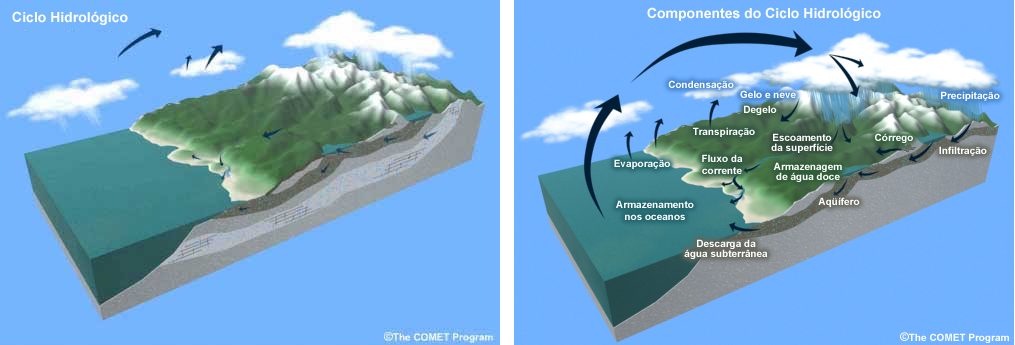
\includegraphics[height=5cm]{./figs/fig01.png}
\caption{Componentes do Ciclo Hidrológico.}
\FONTE{The COMET Program.}
\label{fig01}
\end{figure}

O vapor d'água que ascende proveniente do solo e da vegetação se condensa formando as nuvens. A quantidade e o tipo de precipitação dependem das características do local em que as massas de ar ascendem e formam as nuvens. Nesse caso, a precipitação pode assumir características distintas: Frontal (ocorrendo ao longo da linha imaginária que separa duas massas de ar de características diferentes); Orográfica (em que o ar é forçado a transpor barreiras de montanhas ou encostas íngremes) e Convectiva (precipitação proveniente da ascensão do ar devido às diferenças de temperatura entre duas camadas vizinhas da atmosfera). Além disso, a precipitação é uma variável que se distribui discretamente no tempo e no espaço: ela pode não possuir continuidade de um ponto a outro (pode chover em um local e em outro não) e pode ocorrer em diferentes horários durante o dia.

Usualmente, a chuva é medida nas estações de coleta de dados em superfície através de pluviômetros ou pluviógrafos (aparelhos receptores de água precipitada que registram a altura da chuva no decorrer do tempo). A precipitação pode também ser estimada através de modelos e, de forma remota, através de satélites e radares (capazes de estimar o tipo de nuvens e a quantidade de precipitação em nuvens isoladas e em sistemas convectivos através da temperatura do brilho do topo das nuvens e a partir de imagens de satélites). No entanto, a quantidade de radares meteorológicos e de pluviômetros instalados sobre a superfície do globo, é insuficiente para se determinar de forma contínua a distribuição da precipitação. Com isso, os satélites de sensoriamento remoto são utilizados com diversas aplicações, sendo uma delas a estimativa espaço-temporal da precipitação sobre grandes áreas. Um exemplo deste tipo de aplicação é o satélite TRMM (Tropical Rainfall Measuring Mission) que é capaz de fornecer estimativas de precipitação em alta resolução espaço-temporal (tal como requerem os modelos de previsão). Mesmo assim, observa-se que este tipo de estimativa provê uma amostragem da precipitação que pode não ser contínua no tempo sobre uma mesma área do globo, devido à órbita desses satélites. Recentemente, novos projetos, como o GPM (Global Precipitation Measurement) têm surgido com a expectativa de se utilizar a maior quantidade possível de satélites que tenham a capacidade de fornecer dados a patir dos quais seja possível descrever com precisão a variação espaço-temporal da precipitação, sobretudo sobre a região tropical. Estes projetos surgem para como iniciativa de se tentar resolver um dos problemas críticos da meteorologia atualmente.

Na modelagem atmosférica, a precipitação é diagnosticada pelos modelos de previsão, basicamente, através de parametrizações nas escalas de grade e sub-grade. Na escala de grade são resolvidas a precipitação de larga escala ou estratiforme. Na escala de sub-grade, são tratadas a precipitação associada à convecção rasa (aquecimento diabático, liberação de calor latente) e profunda (chuvas convectivas). Além disso, o diagnóstico preciso da precipitação depende também de uma rede de dados observacionais consistente, a partir da qual seja possível obter informações consistentes para uso com os modelos de previsão. De outra forma, através da modelagem numérica, a precipitação também pode ser estimada através do acoplamento de variáveis prognosticadas pelo modelo Eta (e.g., ventos, umidade relativa, água precipitável) às informações providas pelos satélites. Este tipo de modelagem permite melhorar a representação das estimativas da precipitação.

Este quadro se constitui como um grande desafio para a PNT, principalmente para a previsão de precipitação.

Situada entre os oceanos Pacífico e Atlântico e meridionalmente entre a faixa tropical de latitudes 10ºN e 60ºS, a AS é uma região sobre a qual atuam diversos tipos de sistemas atmosféricos reguladores do tempo e do clima. Dentre eles, pode-se citar: a Zona de Convergência do Atlântico Sul (ZCAS), Zona de Convergência Intertropical (ZCIT), Jatos de Baixos Níveis (JBN) e altos níveis como o Jato Polar Norte (JPN), Jato Polar Sul (JPS) e o Jato Subtropical (JS), Alta da Bolívia e a Baixa do Chaco. Além disso, massas de ar e frentes atmosféricas entram e saem com frequência do continente. O deserto do Atacama, a cordilheira dos Andes, a floresta Amazônica e o Nordeste brasileiro, também são exemplos da diversidade de cenários que compõem a AS - Figura 1.1 (SATYAMURTY et al, 1998).

\begin{figure}
\centering
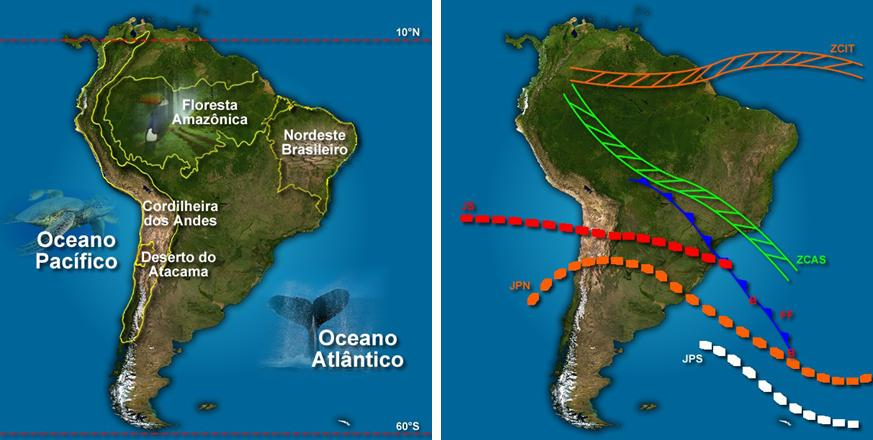
\includegraphics[height=7.5cm]{./figs/fig02.png}
\caption{Os diferentes cenários da América do Sul.}
\label{fig02}
\end{figure}

Toda essa variedade de sistemas ambientais e meteorológicos em um continente situado numa zona tropical do globo é consequência direta dos diferentes regimes de chuva presentes na região, que contribui para a complexidade da PNT.

Além disso, há que se considerar que, pelo fato de a AS estar situada no Hemisfério Sul (HS), as porções de terras e continentes nesta parte do globo são menores do que as porções de mares e oceanos. Esta situação é contrária ao que ocorre no Hemisfério Norte (HN). Nesta parte, a cobertura de radiossondagens e de equipamentos de monitoramento atmosférico (radares) sobre os continentes compõem uma estrutura muito densa mais eficiente de observações. Segundo MOREL (1980) e KALNAY (2003), em um período de aproximadamente 3 horas, a quantidade de informações coletadas (sobre a superfície, atmosfera, mares e oceanos) é insuficiente para iniciar um modelo de Equações Primitivas (equações 1.0, 1.1 e 1.2). Esta diferença, em relação ao número de graus de liberdade desse tipo de modelo, pode chegar a ser de uma ou até duas ordens de magnitude. Este fato indica que atualmente, com modelos mais sofisticados e a altas resoluções, existe uma necessidade muito grande de mais observações. Na prática, este tem sido um dos grandes desafios para a PNT. 

Sobre a AS, em uma janela de 6 horas (para os horários das 00Z e 12Z), há aproximadamente 103 observações convencionais (Figura 1.2), das quais 45\% são observações de radiossondas (pontos em azul claro), 1,5\% são informações de navios (altura geopotencial - pontos vermelhos), 48\% são observações SYNOP (altura geopotencial - pontos azuis), 4\% são observações de boias (altura geopotencial - pontos amarelos) e 1,4\% são observações de aviões (vento - pontos verdes). Para os horários das 06Z e 18Z, a quantidade de observações é sensivelmente menor: há aproximadamente 102 observações (uma ordem de magnitude menor do que nos horários das 00Z e 12Z), sendo 0\% de radiossondas, 5\% de navios (altura geopotencial), 69\% SYNOP, 18\% boias e 7,5\% de informações de vento advindas de aeronaves.

\begin{figure}
\centering
\includegraphics[height=20cm]{./figs/fig03.png}
\caption{Observações convencionais sobre a AS para o dia 28 de setembro de 2009, assimiladas pelo sistema RPSAS. Estas observações são válidas para os horários das 00Z e 12Z (primeira linha) e para o horário das 06Z e 18Z (segunda linha).}
\FONTE{http://assimila.cptec.inpe.br}
\label{fig03}
\end{figure}

Na modelagem atmosférica, o aprimoramento da PNT de curto e médio prazo depende não somente do poder computacional envolvido - supercomputadores cada vez mais rápidos e eficientes (que permitem calcular as previsões de tempo mais rapidamente ou mesmo aumentar a resolução dos modelos), mas principalmente de fatores como o conhecimento exato das leis que governam o movimento da atmosfera, da quantidade de dados observacionais e da determinação do estado inicial da atmosfera.  Embora não se tenha um conhecimento total sobre estas leis e condições - pois a atmosfera possui uma previsibilidade limitada (devido ao seu comportamento caótico), os modelos de PNT são fundamentados na estrutura básica da atmosfera (leis de conservação de movimento, termodinâmica e continuidade - equações 1.0, 1.1 e 1.2). Desta forma, tais modelos mantêm forte dependência em relação às condições do estado inicial da atmosfera, um importante fator que torna possível a previsão numérica de tempo mais acurada. Este fator - a condição inicial, também chamada de análise na assimilação de dados, é determinante para a PNT: quanto mais completo for - quanto mais informações possuir sobre o fluxo da atmosfera em seu instante de análise, mais preciso (acurado) será o resultado da previsão. (Convenciona-se, a partir daqui, que os vetores são denotados em negrito e as matrizes em letras maiúsculas).

\begin{equation}
\frac{d\textbf{\textit{v}}}{dt}+\textbf{\textit{v}}\cdot\nabla\textbf{\textit{v}}+2\Omega\times\textbf{\textit{v}}=-\frac{1}{\rho}\nabla{p}+\textbf{\textit{g}}+\textbf{\textit{f}}
\label{form01}
\end{equation}

\begin{equation}
\frac{d\rho}{dt}+\nabla\cdot(\rho\textbf{\textit{v}})=0\rightarrow\frac{d\rho}{dt}=-\nabla\cdot(\rho\textbf{\textit{v}})
\label{form02}
\end{equation}

\begin{equation}
\frac{D\textit{e}}{D\textit{t}}=-\rho\frac{D\alpha}{D\textit{t}}+\textit{Q}
\label{form03}
\end{equation}

Onde:

\begin{itemize}
\item \textbf{\textit{v}}: é o vetor velocidade do fluido atmosférico em três dimensões, num referencial rotacional;
\item $\Omega$: é o vetor tridimensional velocidade angular (velocidade com a qual o referencial rotacional se move);
\item $\rho$: é a densidade do fluido atmosférico;
\item \textit{p}: é a pressão do fluido atmosférico;
\item \textbf{\textit{g}}: é o vetor aceleração gravitacional em três dimensões;
\item \textbf{\textit{f}}: representa o vetor tridimensional da força de atrito (entre a atmosfera e a superfície terrestre);
\item \textit{e}: é a energia interna específica, que é uma função da temperatura do sistema;
\item \textit{Q}: é calor por unidade de massa;
\item $\alpha$: volume específico do fluido atmosférico. 
\end{itemize}

KRISHNAMURTY et al. (1991) e NUNES e ROADS (2005) apontam para o fato de que uma previsão acurada de precipitação na região dos trópicos está diretamente relacionada com a qualidade dos campos iniciais de temperatura e umidade do solo, sem os quais os fluxos de calor necessários para a correta simulação/composição da estrutura vertical das nuvens convectivas é comprometida.

Nesse sentido, a assimilação de precipitação tem sido proposta como uma forma capaz de representar melhor esses campos iniciais - quanto mais realísticos, melhor será a simulação/representação da convecção, a formação de nuvens e precipitação. Isto permite reduzir o tempo de spin-up (tempo necessário para que se ajustem dinamicamente as condições iniciais aos campos prognósticos do modelo), incrementando a qualidade das análises globais e das previsões de curto prazo sobre os trópicos (HECKLEY et al., 1990; FALKOVICH et al., 2000).

Outros trabalhos mostram também que a utilização da assimilação de precipitação para a inicialização dos modelos é mais substancial para o aprimoramento da qualidade das previsões de curto prazo, uma vez que esta é vinculada às parametrizações físicas (como esquemas de convecção) e aos erros sistemáticos do modelo (KASAHARA et al., 1994; MATHUR, 1995; ZUPANSKI E MESINGER, 1995; NUNES E COCKE, 2004; MESSINGER et al., 2005.

Tendo-se em vista que nas regiões tropicais do globo a convecção tem um papel dominante e sabendo-se que, em geral, os dados provenientes de radiossondagem têm baixa resolução espacial e temporal (cobertura de aproximadamente de 300 km na horizontal e 10 km na vertical e 1 h de duração), dificilmente consegue-se uma boa interpolação em mesoescala. Consequentemente a convecção tende a não se formar nos horários e locais previstos por um modelo de mesoescala (como é o caso do Eta). Uma forma de se corrigir ou contornar este problema é incluir a precipitação no ciclo de assimilação de dados. A assimilação de precipitação utilizada nesta dissertação de mestrado segue um esquema de Inicialização Física (IF), no qual são ajustados os campos de precipitação do modelo de acordo com os campos de precipitação observados do TRMM. Maiores detalhes sobre este procedimento são mostrados no Capítulo 2, bem como a revisão bibliográfica sobre o assunto. No Capítulo 3 é apresentada a descrição dos dados utilizados e da metodologia empregada. No Capítulo 4, são apresentados os resultados obtidos com a assimilação de precipitação e, no Capítulo 5, as conclusões.

\section{Objetivos}
\label{ss:objetivos} 

\textbf{Objetivo Geral:}

O objetivo principal deste trabalho é avaliar o impacto da inclusão de dados de precipitação no sistema de assimilação de dados regional do CPTEC. Para este propósito será usado o sistema de assimilação de dados RPSAS junto com o modelo regional de mesoescala EtaWS.

\textbf{Objetivos Específicos:}

\begin{itemize}
\item Realização de experimentos com e sem assimilação de precipitação;
\item Avaliação do impacto da assimilação de precipitação e avaliação do skill do modelo;
\item Estudos de casos de CCMs ocorridos em janeiro de 2003: identificação e simulação (ciclo de vida, posicionamento e intensidade).
\end{itemize}
